\begin{tcolorbox}
\chapter{2011 - Izgubljeni Raj}

2011 was another great year deep within \passage[mountain]{Tolminski Migovec}. The weather
was horrendous -- we even had snow! But the cave kept on going. We
found over 2.2 km of new passage all below -500 m in depth, and took the
cave to a new deepest point of -888 m. All of the exploration took place
during underground-camping trips based at \passage{X-Ray}
(\passage{Vrtnarija}, -550 m), with the keenest of expeditioneers managing
a total of around seven nights underground during the four week
expedition.

'Izgubljeni Raj' quite simply translates as 'Paradise Lost', a reference to the beautiful crystals found in the \passage{Palace of King Minos} during 2010.

\end{tcolorbox}
\backgroundsetup{
    scale=1,
    color=black,
    opacity=1,
    angle=0,
    contents={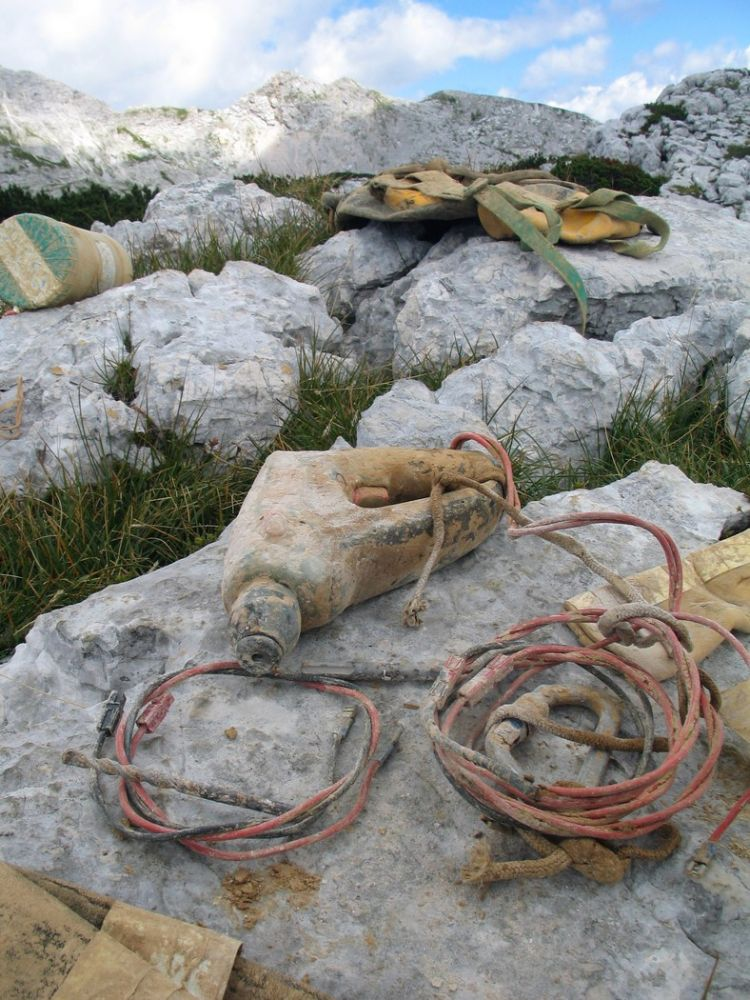
\includegraphics[height=\paperheight]{2011/intro/2011-08-10-11.38.42-Jarvist Frost-CanonG5-IMG_0188 - Drying Underground Camp gear in the Sun--orig_1050p.jpg}}
}
\BgThispage









